

\chapter{Epidermal Robots}
This chapter describes the design and manufacturing of Epidermal robots.  Also, it attempts to rationalize the design decisions of the robot. The first functional Epidermal robot is called SkinBot, and is the main focus of this chapter. 
In the future Epidermal robots should be made from soft materials, so they match the elasticity of the skin and are more resilient. The soft robotics prototype is briefly described at the end of the chapter.

\section{Introduction}
To perform their tasks successfully, Epidermal robots need to meet several specific requirements. First, the robots need to be \textbf{lightweight and small} (under 80 grams and centimeter-sized according to our experiments) to minimally disrupt the person while exploring the different parts of the body. Second, Epidermal robots need to have direct \textbf{access to the skin}. Human skin is not only the largest organ of the human body but also offers a good proxy to capture relevant information about the outer skin (e.g., appearance, texture) and inner body responses such as physiological signals (e.g., electrocardiograms, electrodermal activity). Third, the robot needs the \textbf{ability to adhere and locomote} over the non-uniform skin, which contains many irregularities such as wrinkles, joints, and hair. Moreover, the locomotion should be robust to different robot orientations. Forth, epidermal robots should offer \textbf{multimodal sensing}. The human body contains a large range of information that requires different types of sensing modalities. To ensure the robot can successfully digitize the human body, the sensing module should contain as many sensors as possible while still satisfying the previous considerations. Finally, epidermal robots should have the ability of accurate \textbf{self-localization} on the body (under 18 mm. error rate), which is key for autonomous operation and mapping of the human body.
%\section{Previous commitment}
\section{Implementation}
For reference and reproduction, all the design files and software can be found in an online repository\footnote{https://github.com/adementyev/SkinBot}.

\subsection{Skin Adhesion}
Human skin has complex mechanical behavior and is elastic at small loads. In particular, with Young's modulus \footnote{Young modulus is a measure of material's stiffness. It is defined by the relation between strain and stress} ranges from about 0.1MPa to 1.1MPa~\cite{diridollou2000vivo}, with a high dependence on the test subject's age and the mechanical model and measurement instrument~\cite{agache1980mechanical}. Also, the human body has some degree of curvature and features such as hair which makes adhesion even more challenging. Since skin is a complex surface, we conduct \textit{in vivo} experiments as much as possible. However, in some cases such as testing specific skin curvature, we perform experiments on artificial skin created with silicone (Ecoflex 00-30, Smooth-On)\footnote{https://www.smooth-on.com/products/ecoflex-00-30/} that has similar Young's modulus to the skin. 

\begin{figure}[!ht]
\centering
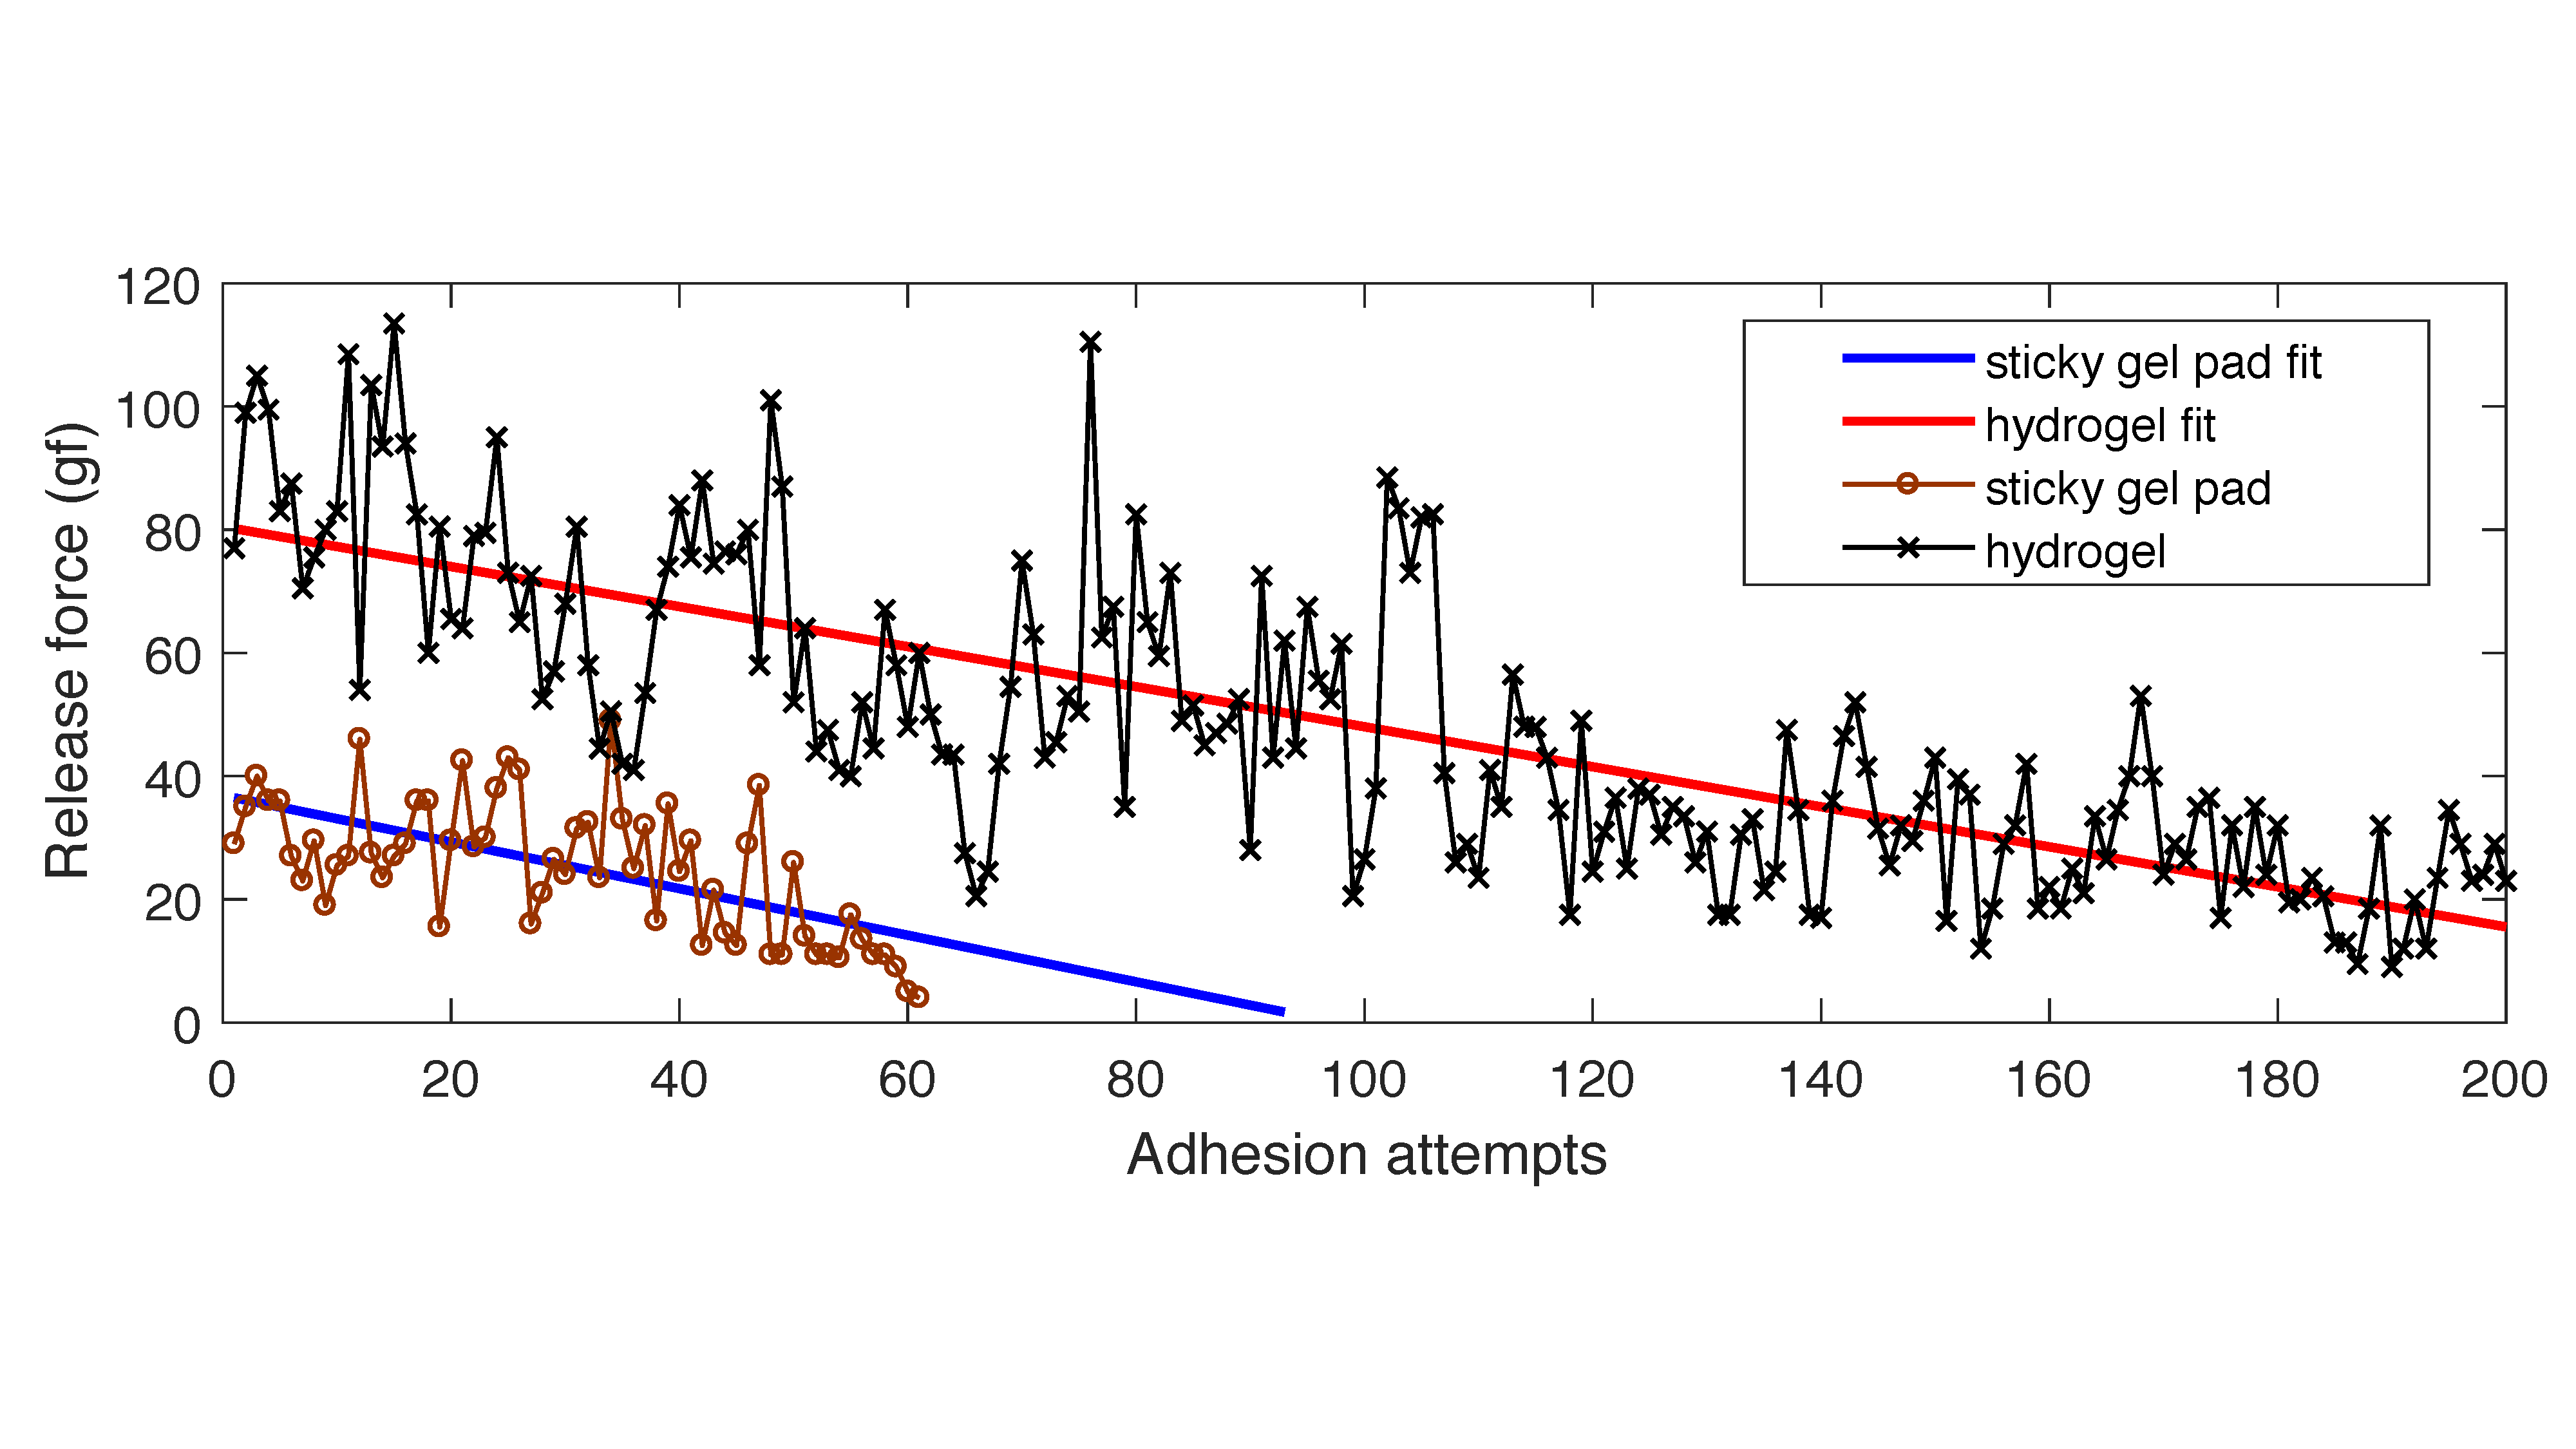
\includegraphics[width=11.0cm]{pictures/chapter3/hydrogel.pdf}
\caption{Test of different adhesives with the skin. Testing of two adhesives for repeated sticking and releasing on the skin. Overlaying the data are lines of the linear fitting. We tested a hydrogel and a sticky gel pad. The hydrogel worked for more adhesions than sticky gel pad, before losing adhesive properties. The release forces had large variations from sample to sample. The testing was conducted with a 20N force gauge, and peak force was recorded.}
\label{fig:hydrogel}
\end{figure}

We designed and built a total of six robot prototypes that considered different locomotion systems (Fig.~\ref{fig:prototypes}). On the one hand, some adhesion approaches such as pinching the skin were not practical and were excluded from the start. On the other hand, adhesive wheels and tracks did not provide consistent adhesion force. For instance, the adhesive force of two commercial adhesives (Katecho and Premium Fixate Cell Pads, CloudValley) decreased with each peel by about half a percent (Fig.~\ref{fig:hydrogel}) while having large variations between peels. With continuous attachment and detachment cycles, required for locomotion, the adhesive force quickly degrades. Also, the hydrogel adhesive picks up dirt, oil and dead epithelial from the skin, thus requiring periodic cleaning. After considering different methods, we finally selected a suction-based approach which was inspired by living organisms such as leeches and cephalopods (e.g., squid, octopus). 

\begin{figure}[!t]
\centering
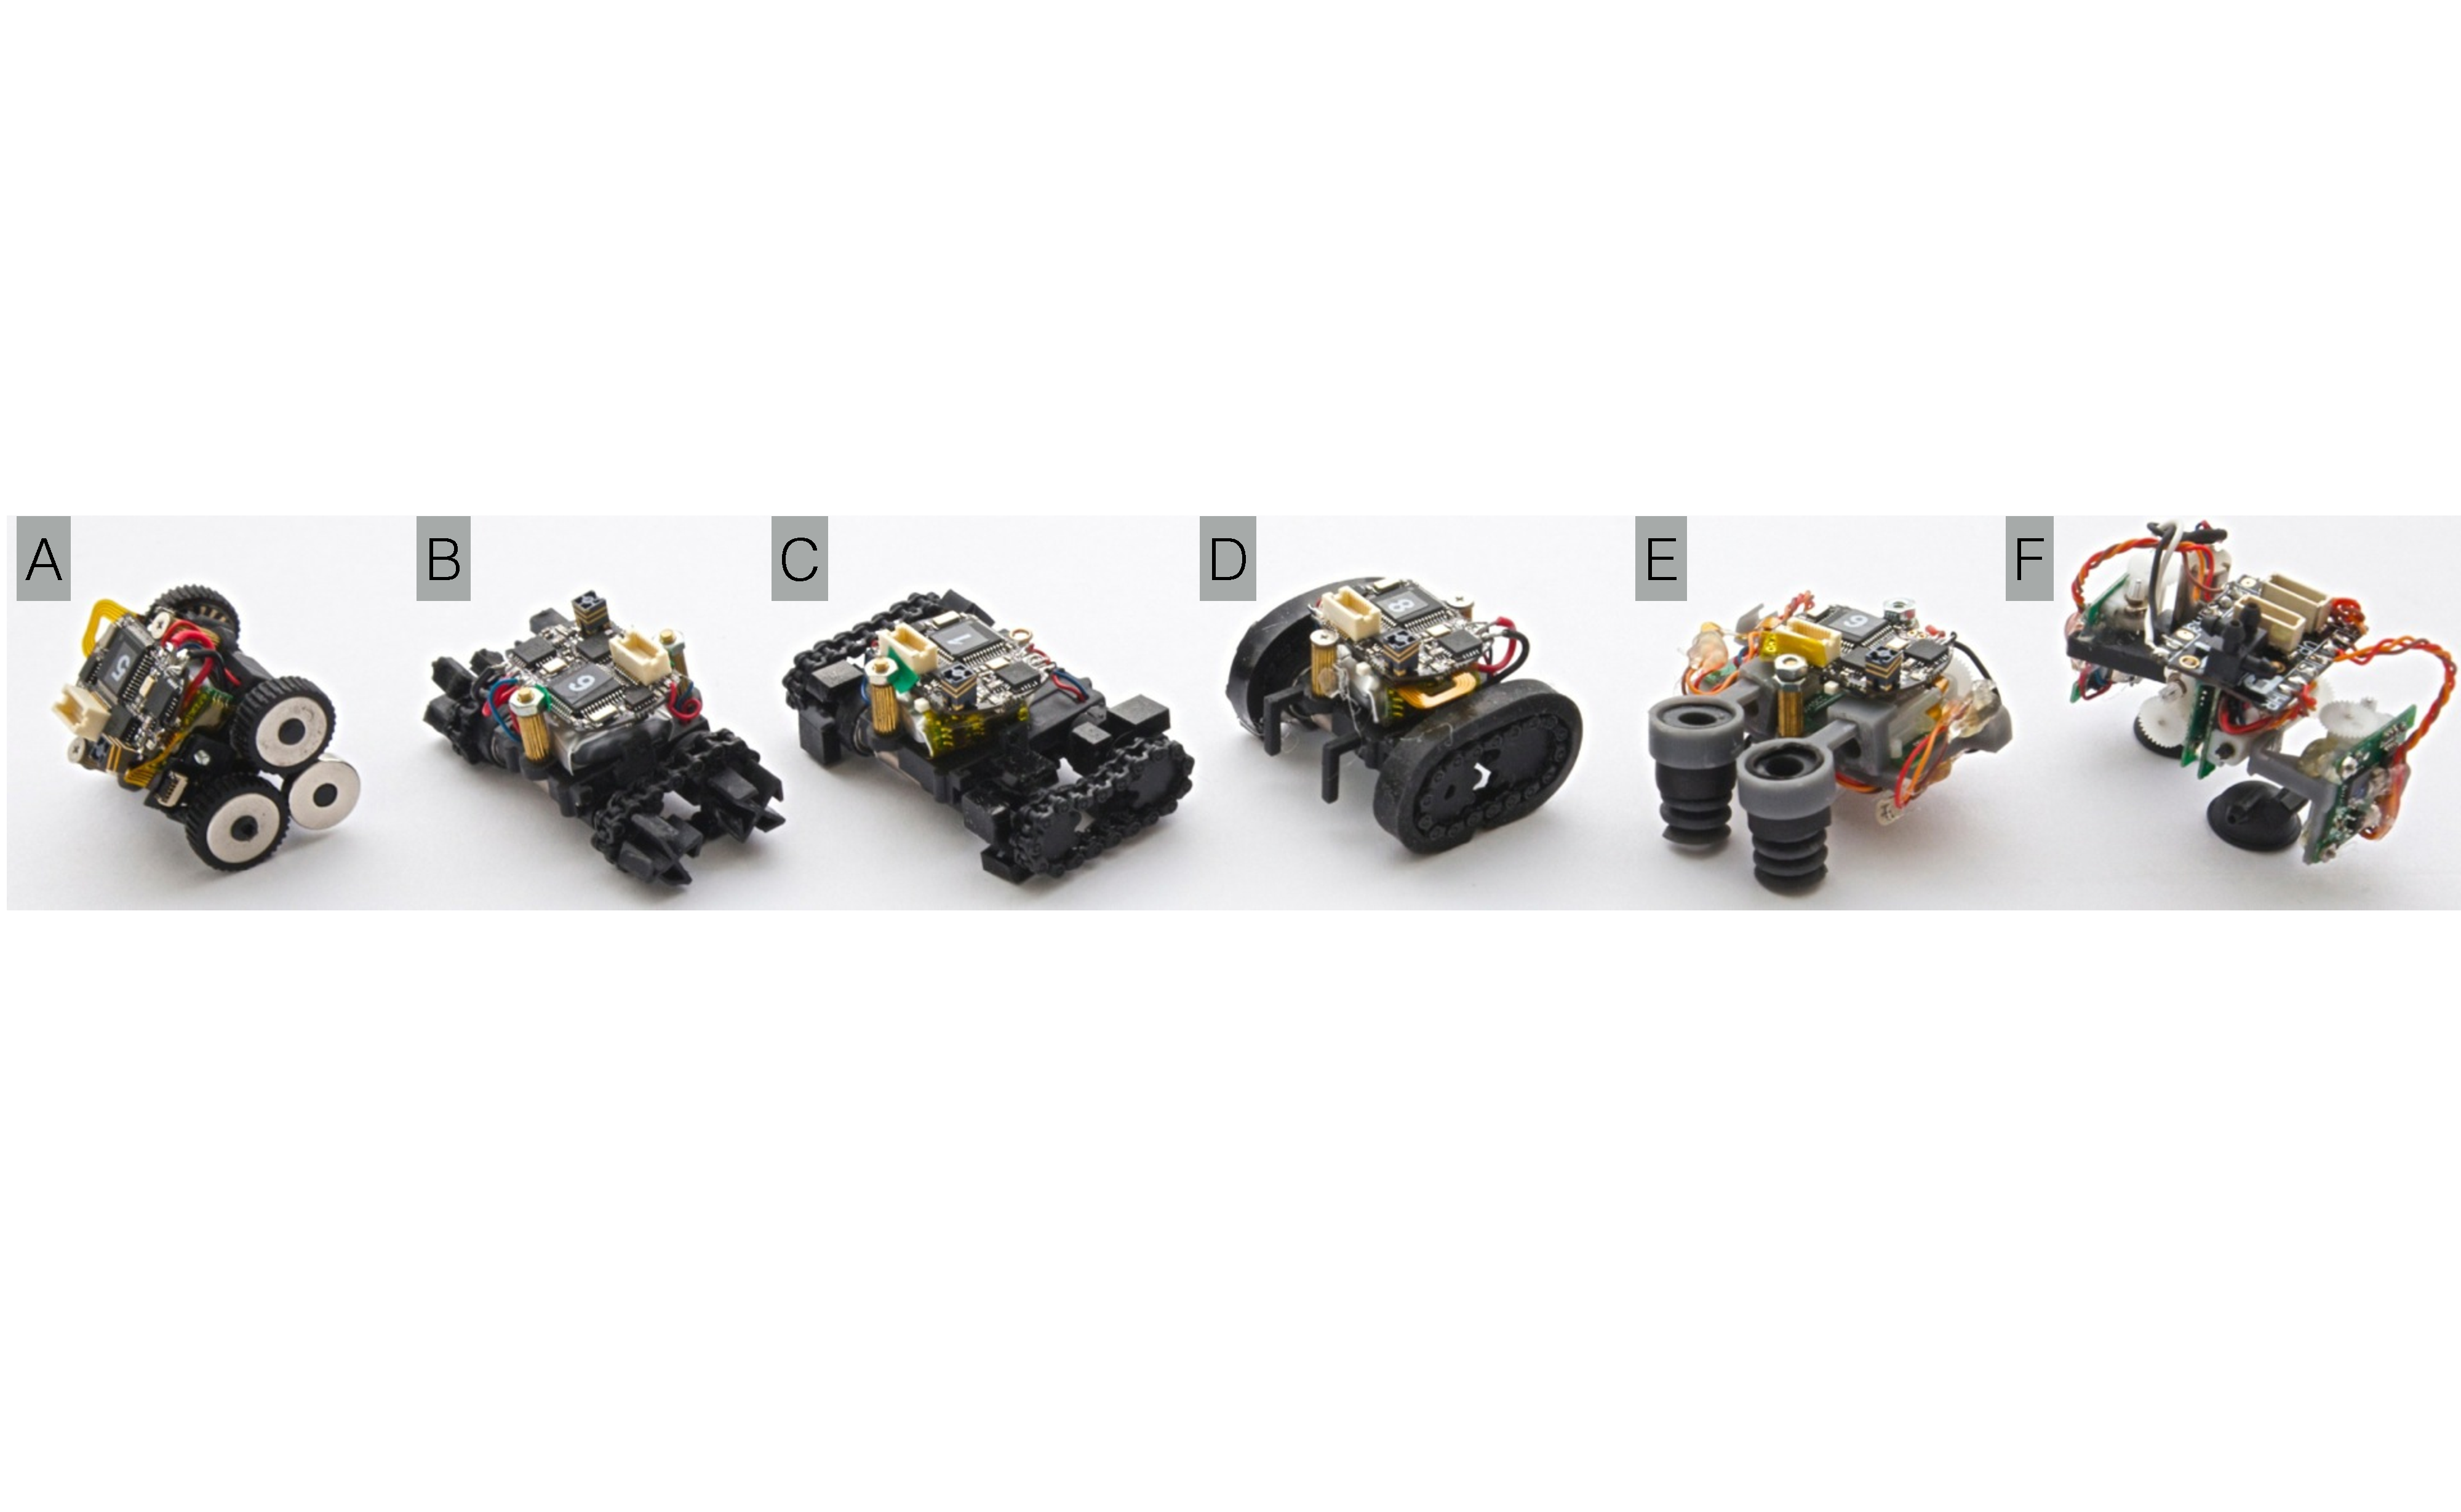
\includegraphics[width=15.8cm]{pictures/chapter3/prototypes.pdf}
\caption{The iterative design process of SkinBot showing different prototypes. A) Rovables ~\cite{dementyev2016rovables}, cloth climbing robot. The initial designs were based on Rovables platform. B)~Prototype based on a wheel-leg climbing robot design in~\cite{daltorio2005small}. Tracks on the outside were used to synchronize the wheels. This prototype does not have enough contact area to reliably adhere to the skin. C)~Similar wheel-leg design, but contains tracks on the inside. This design also does not have enough contact area. D) Prototype with sticky tracks. E)~Initial suction-based robot with two servo motors that allows suction cups to extend and contract. We found that two motors are not enough for reliable movement, as the suctions need to be pushed down to create a reliable seal. F)~Current robot design, which is explained in detail in this paper.}
\label{fig:prototypes}
\end{figure}


In suction-based locomotion, a suction force appears when a lower pressure is created inside a cup and the pushing of the atmospheric pressure causes an adhesion force. While suction cups used in the industrial applications are usually made of soft rubber, we found that rigid cups can be used with the skin. Under vacuum, the flexible skin gets pulled into the cup to seal the skin-cup interface (shown in Fig.~\ref{fig:suction_cup_design}C). While rigid suction cups can be quickly prototyped with a standard 3D printer, flexible suction cups require a multi-part silicone mold. We found that the bell-shaped cup worked well with the skin. The bell provided a large inside volume, into which the skin can expand. Same bell design is often used in cupping therapy, alternative medicine in which suction cups are applied to reduce pain and swelling.   

\begin{figure}[!ht]
\centering
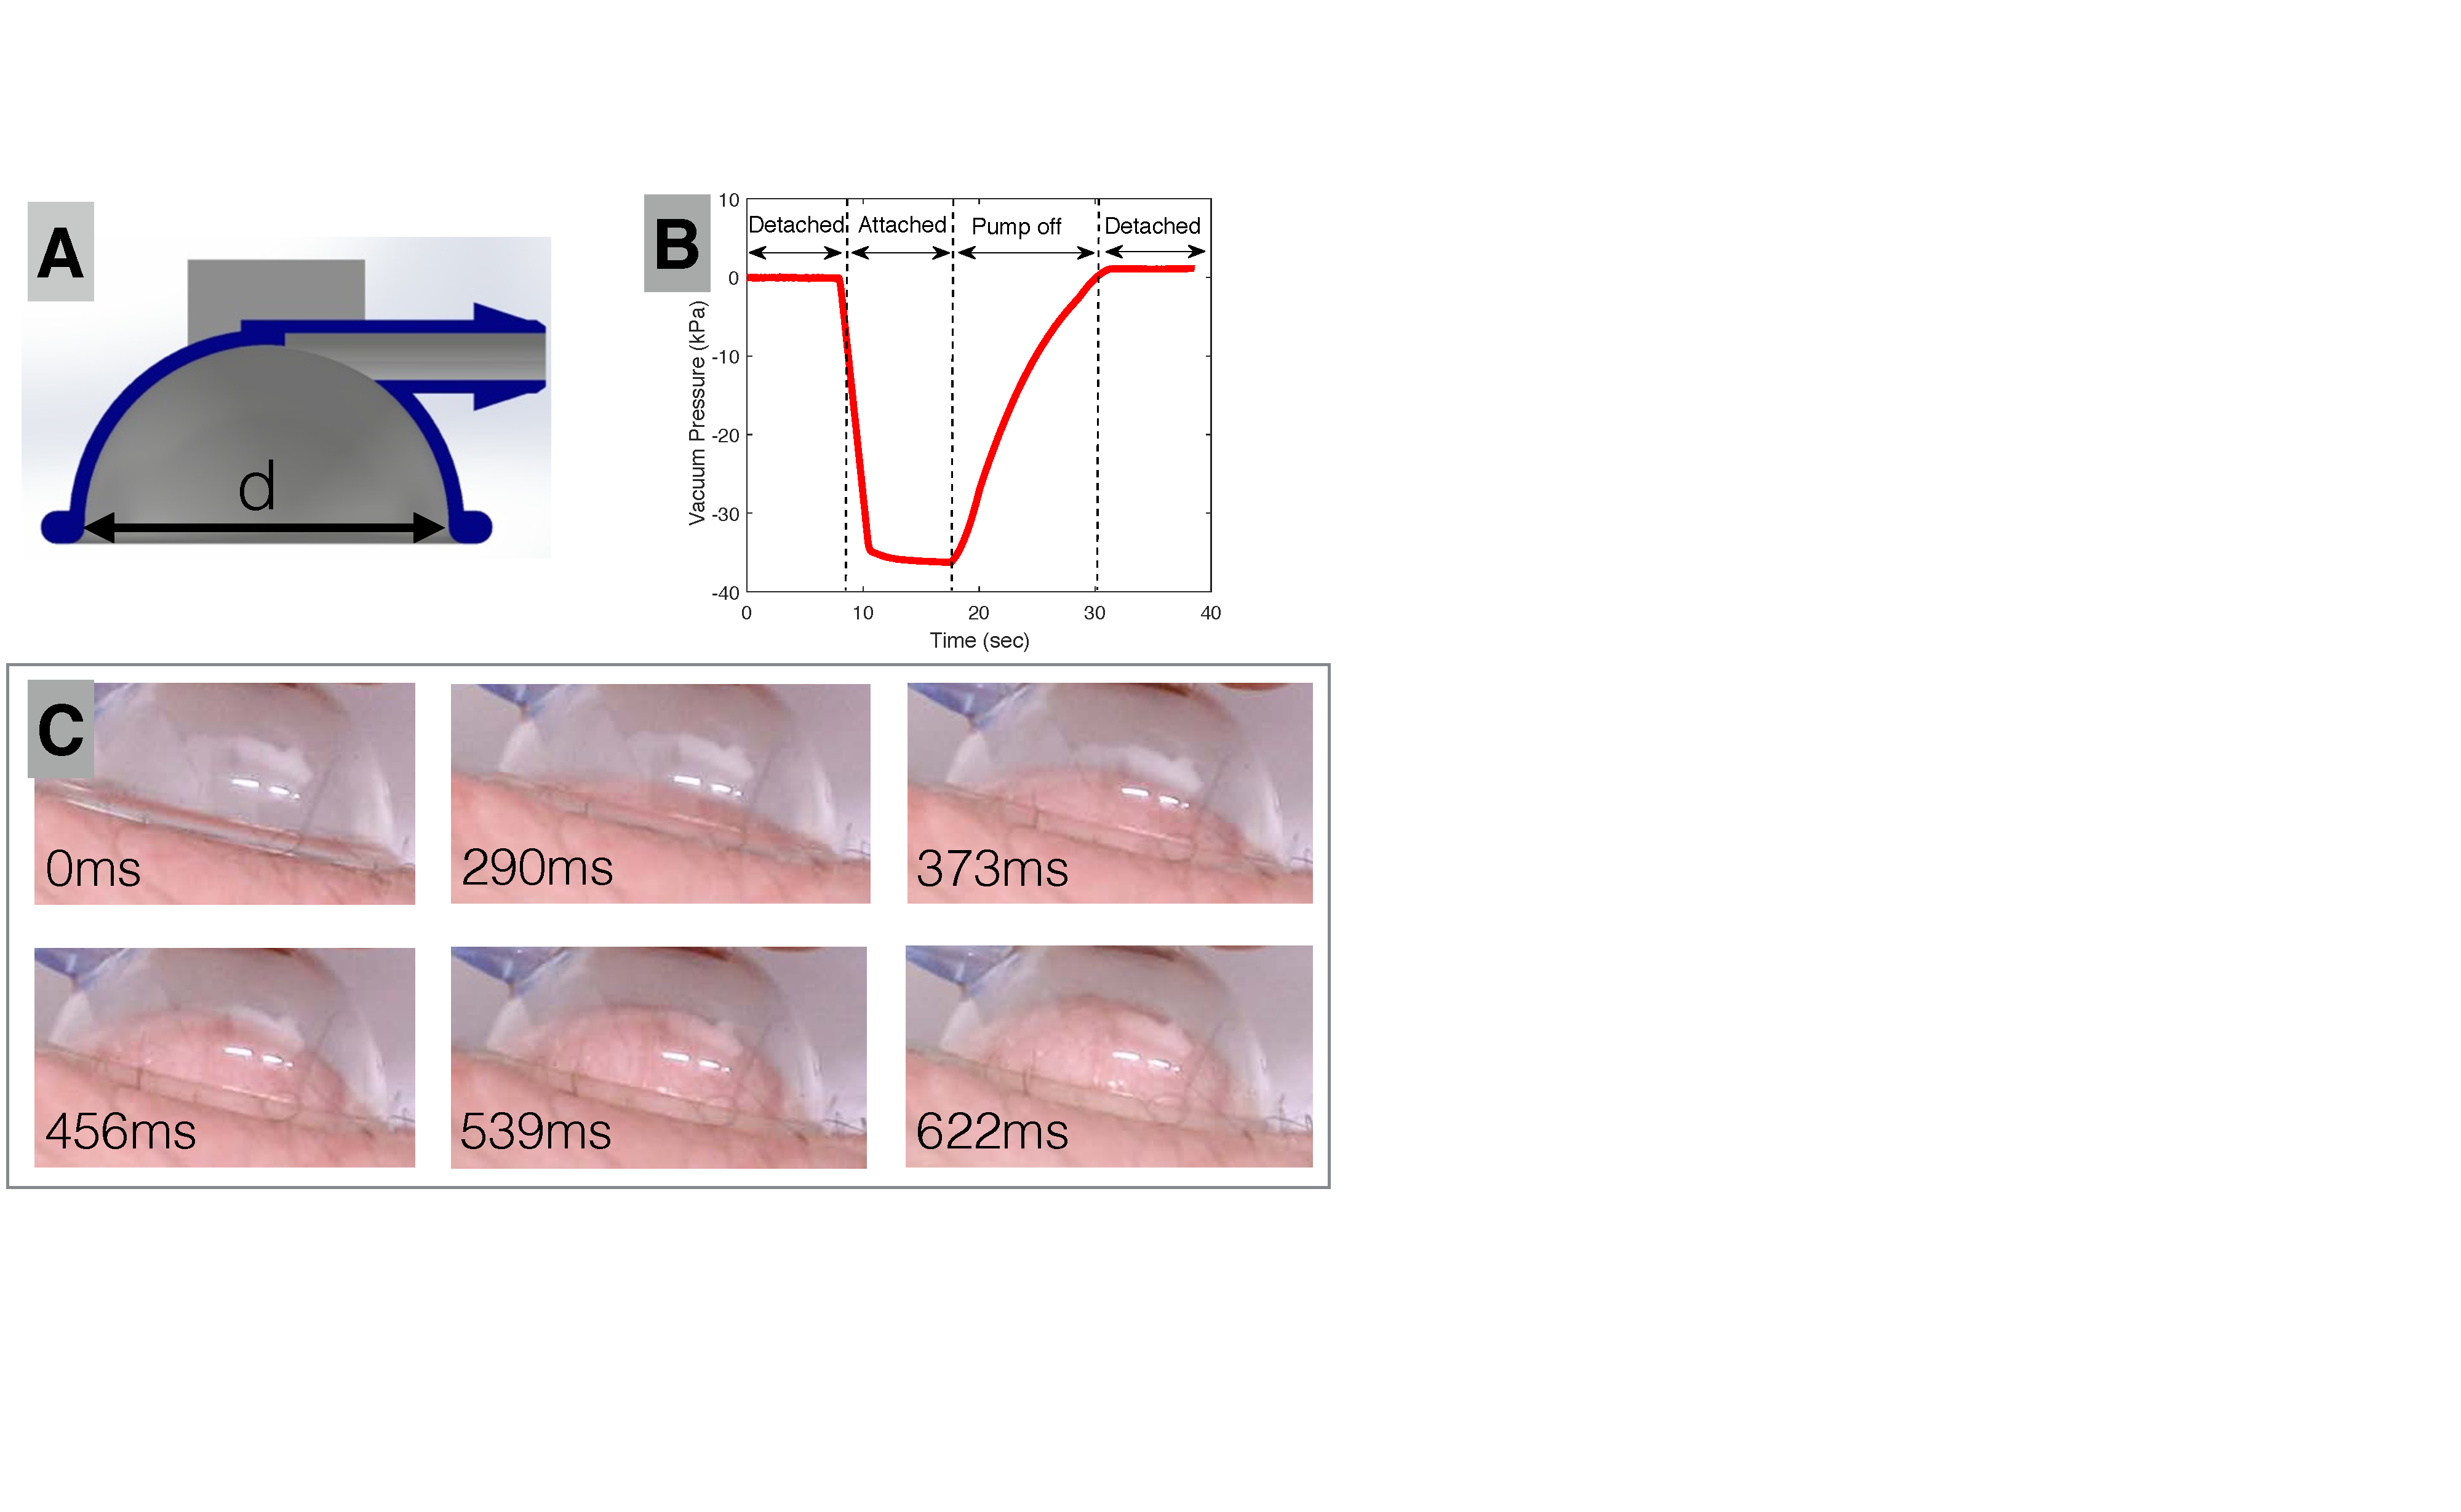
\includegraphics[width=8.9cm]{pictures/chapter3/suction_cup_design_small.pdf}
\caption{Suction cup design for skin attachment. A)~The cross section of the suction cup CAD model. B)~The vacuum pressure changes during the suction cup attachment and detachment. C)~Snapshots of suction cup attachment to the skin. }
\label{fig:suction_cup_design}
\end{figure}

The final implementation of SkinBot uses two 9mm-diameter suction cups. To make the suction cups as well as all other mechanical parts, we used a 3D printer (Form 2, Formlabs, gray resin). The 9mm suction cup provided the best size-to-adhesion-force tradeoff and is analyzed in more detail in the results section. This configuration provided a maximum of 200gf (gram-force) adhesion force which is enough to securely hold 20-gram SkinBot. The minimum vacuum pressure required for skin adhesion was measured to be about -10kPa. However, we pull the maximum vacuum of -30kPa using a small membrane diaphragm pump (SC3101PM, Skookum Electronic co.). This pressure was determined by the construction of the pump, specifically by the piston displacement volume. When the vacuum pump is turned off, due to leakage, the pressure slowly returns to atmospheric pressure. To speed up this process, we added a solenoid valve (S070C-SDG-32, SMC Pneumatics) that vents the vacuum line. Using a diaphragm pump has also some problems such as the loudness (55 dB from 30cm) and the large size (32x8x18mm). We also considered piezoelectric pumps but current commercial models (e.g., mp5, Servoflo) only provide a maximum of -10kPa which does not leave any safety factor for air leaks, hair and pump variations which can make adhesion less reliable. 

\subsection{Skin Locomotion}
We wanted to achieve locomotion with the ability to turn with a minimum number of motors as they are one of the largest components. The selected gait was inspired by an inchworm mechanism where climbing is achieved by creating an anchor point and pushing the body away from that point. At a minimum, this motion requires one actuator, to extend and contract the body. In our case, however, we used two linear servo motors to extend and contract the body to allow independent left and right side control. In particular, we used linear servo motors (SPMSA2005, Spektrum) with a 9.1mm throw, commonly used in small radio controlled airplanes which can pull 100gf (gram-force) and weight around 1.8 grams. Furthermore, at least two independent anchor points are required, which can be detached and attached on demand. Thus, two independent pumps and suction cups were used to provide controllable attachment. Also, we added two of the same linear motors to move the suction cups up and down. This prevented dragging of the end effector during extension and contraction and gave the robot the ability to attach to non-uniform surfaces. Finally, we added a planetary gear motor (TGPP06-D-136, TT Motor) and a motor controller (DRV8835, Texas Instruments) to add turning ability around one of the suction cups. 

One of the key challenges with skin locomotion is to ensure reliable adhesion in the new end effector position. To address this, we added an air pressure sensor (MPXV611, NXP) in each of the vacuum lines to detect if the suction cup is attached. The pressure data were collected at 100Hz and filtered by a moving average of 20 samples to remove oscillations of the pump. The attachment was insured by moving the suction cup down in small increments and checking for adhesion each time. The whole locomotion was controlled by a finite state machine with 6 states and was implemented on an ARM Cortex M3 microcontroller (Teensy 3.6, PJRC). As shown in Fig.~\ref{fig:locomotion_mechanism}A, the transitions of the state machine were controlled by the pressure sensors. We conducted the testing using a tethered prototype which contained valves, pumps, power and control electronics on a separate master board, shown in Fig.~\ref{fig:master_node}. The overall system architecture is shown in Fig.~\ref{fig:system_diagram}A. 

\begin{figure}[!ht]
\centering
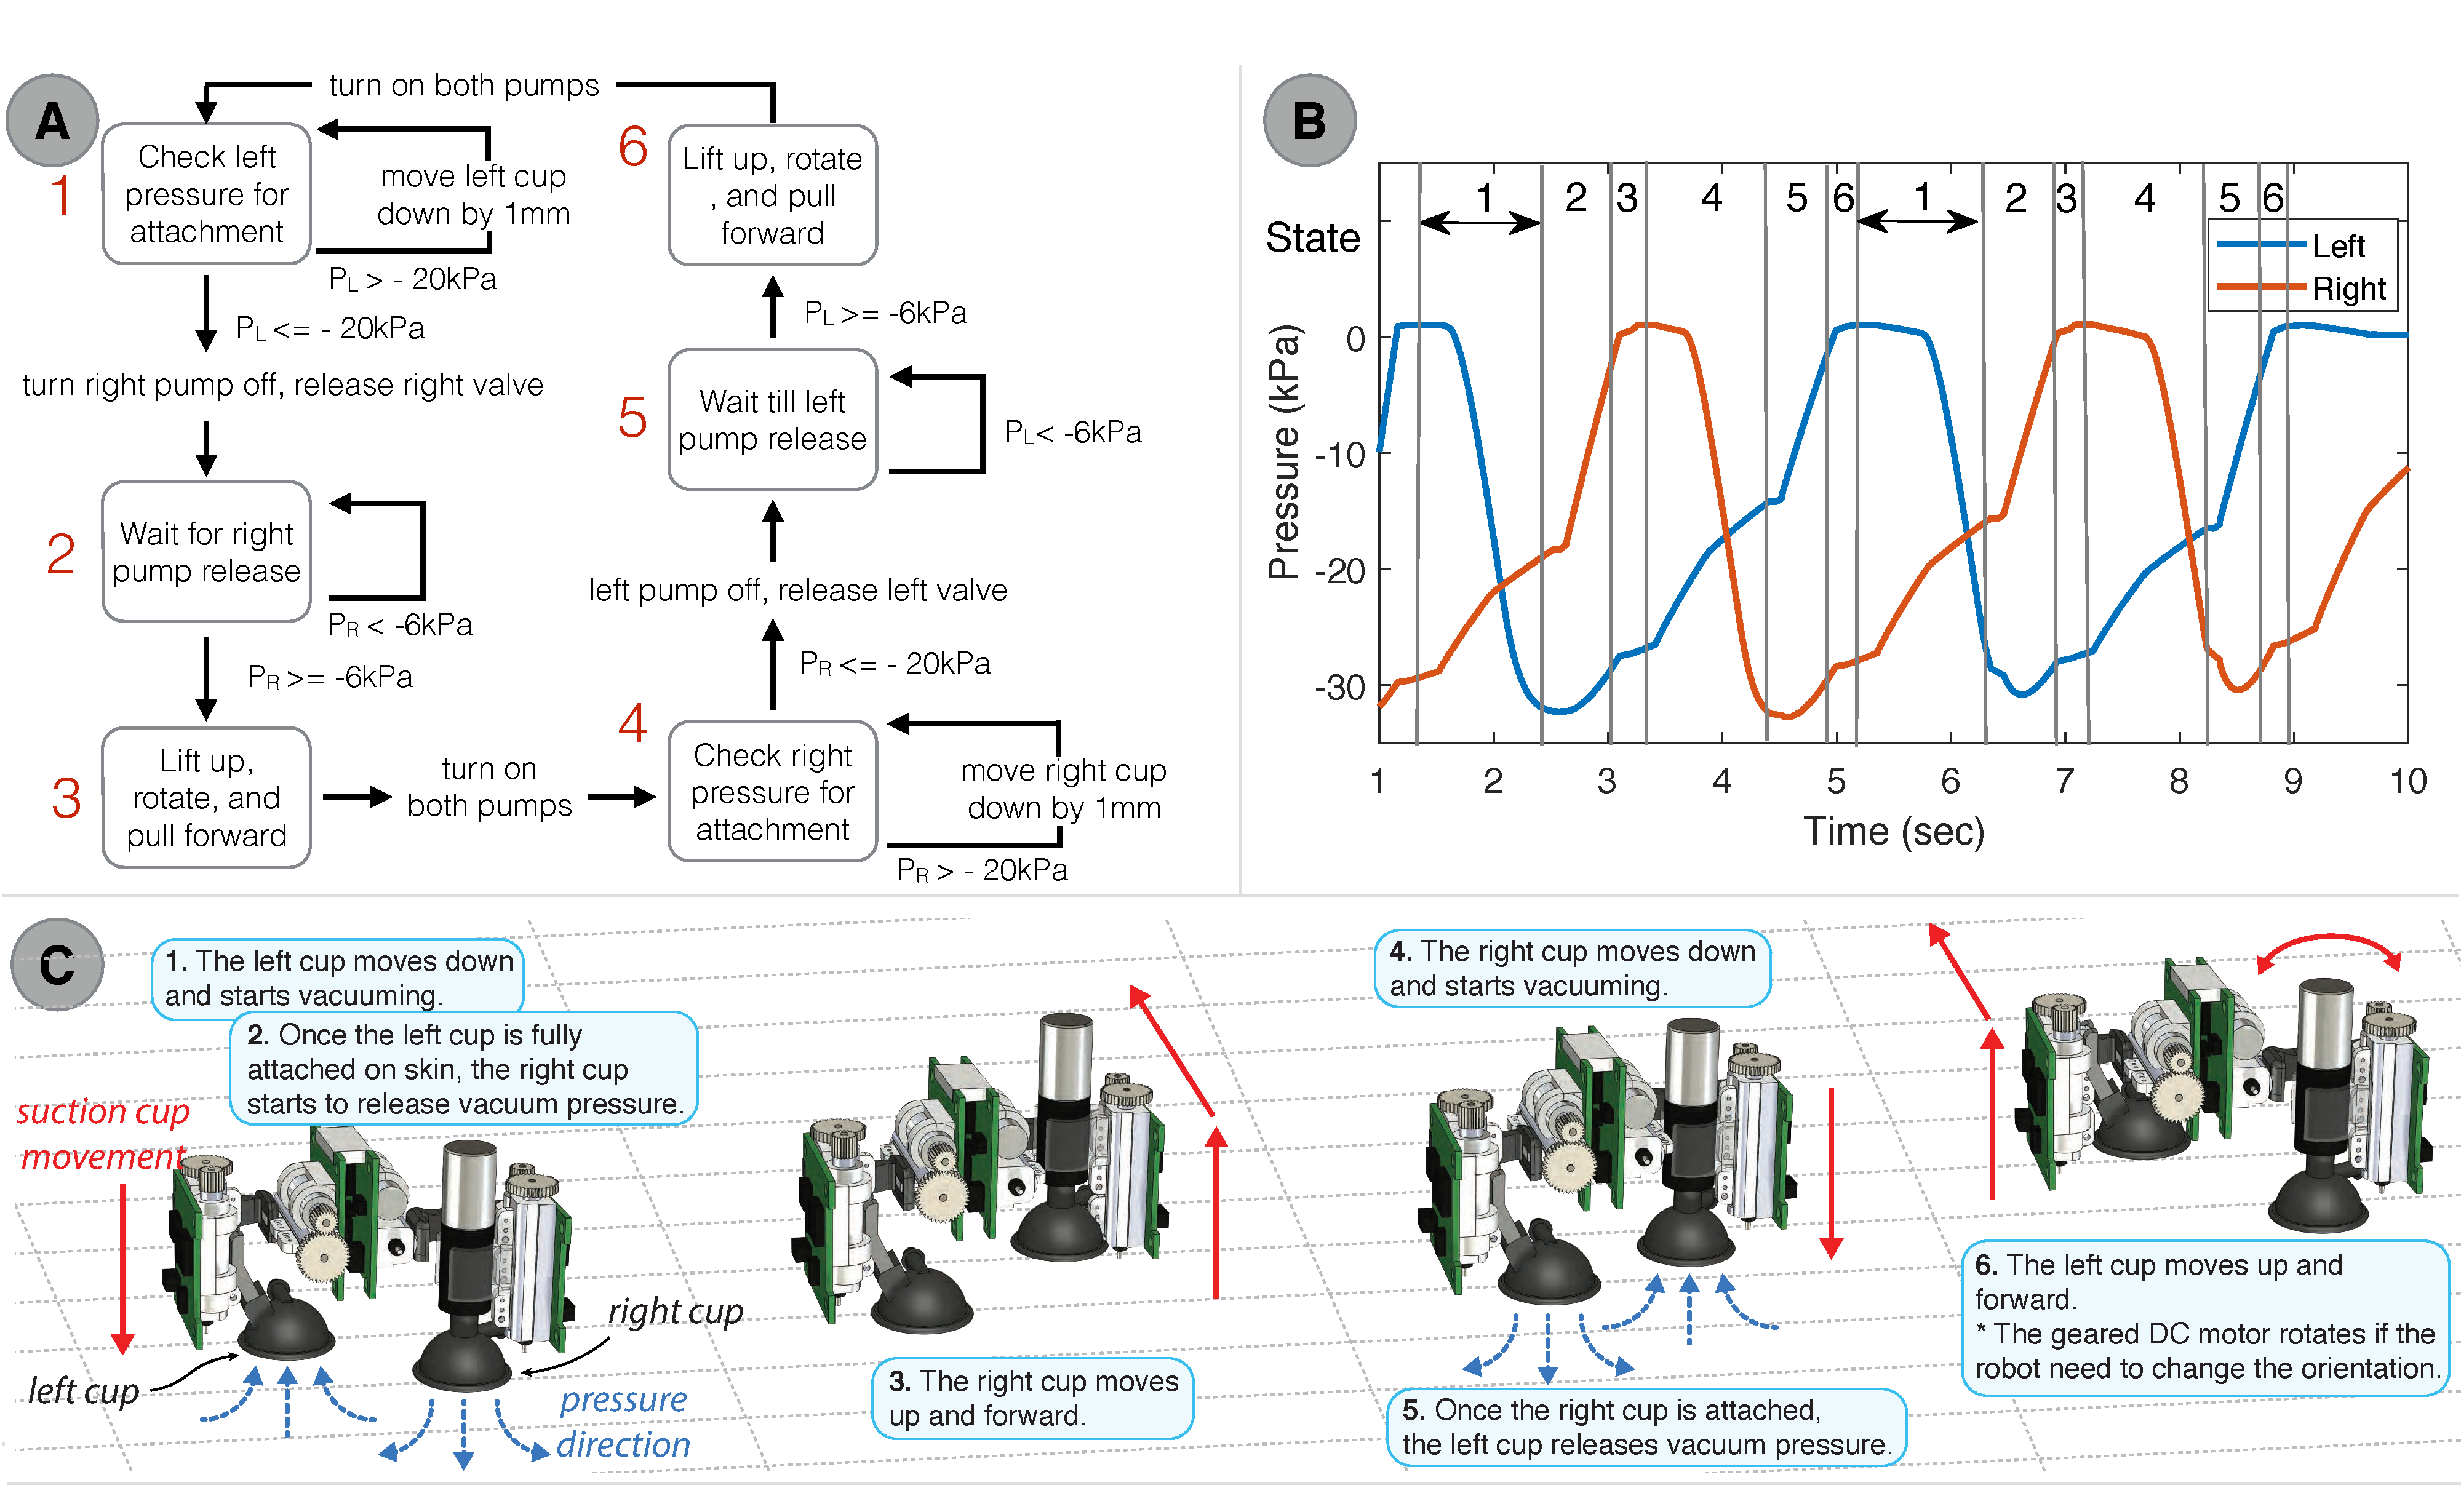
\includegraphics[width=14.0cm]{pictures/chapter3/locomotion_mechanism.pdf}
\caption{Locomotion mechanism overview. A)~Finite state machine diagram for the robot locomotion. The rounded rectangles and arrows represent the states and transitions, respectively. The red numbers next to the circles indicate specific states. The pressure sensors control the state machine. States 1 and 4 involved reattaching suction cups, which was done by moving the suction cup down in increments and checking the pressure each time. B)~Pressure changes during the locomotion sequence, which was measured independently on the right and the left suction cups. The diagram also shows the corresponding states of the finite state machine on the top. C)~Model representing physical locomotion.}
\label{fig:locomotion_mechanism}
\end{figure}


\begin{figure}[!ht]
\centering
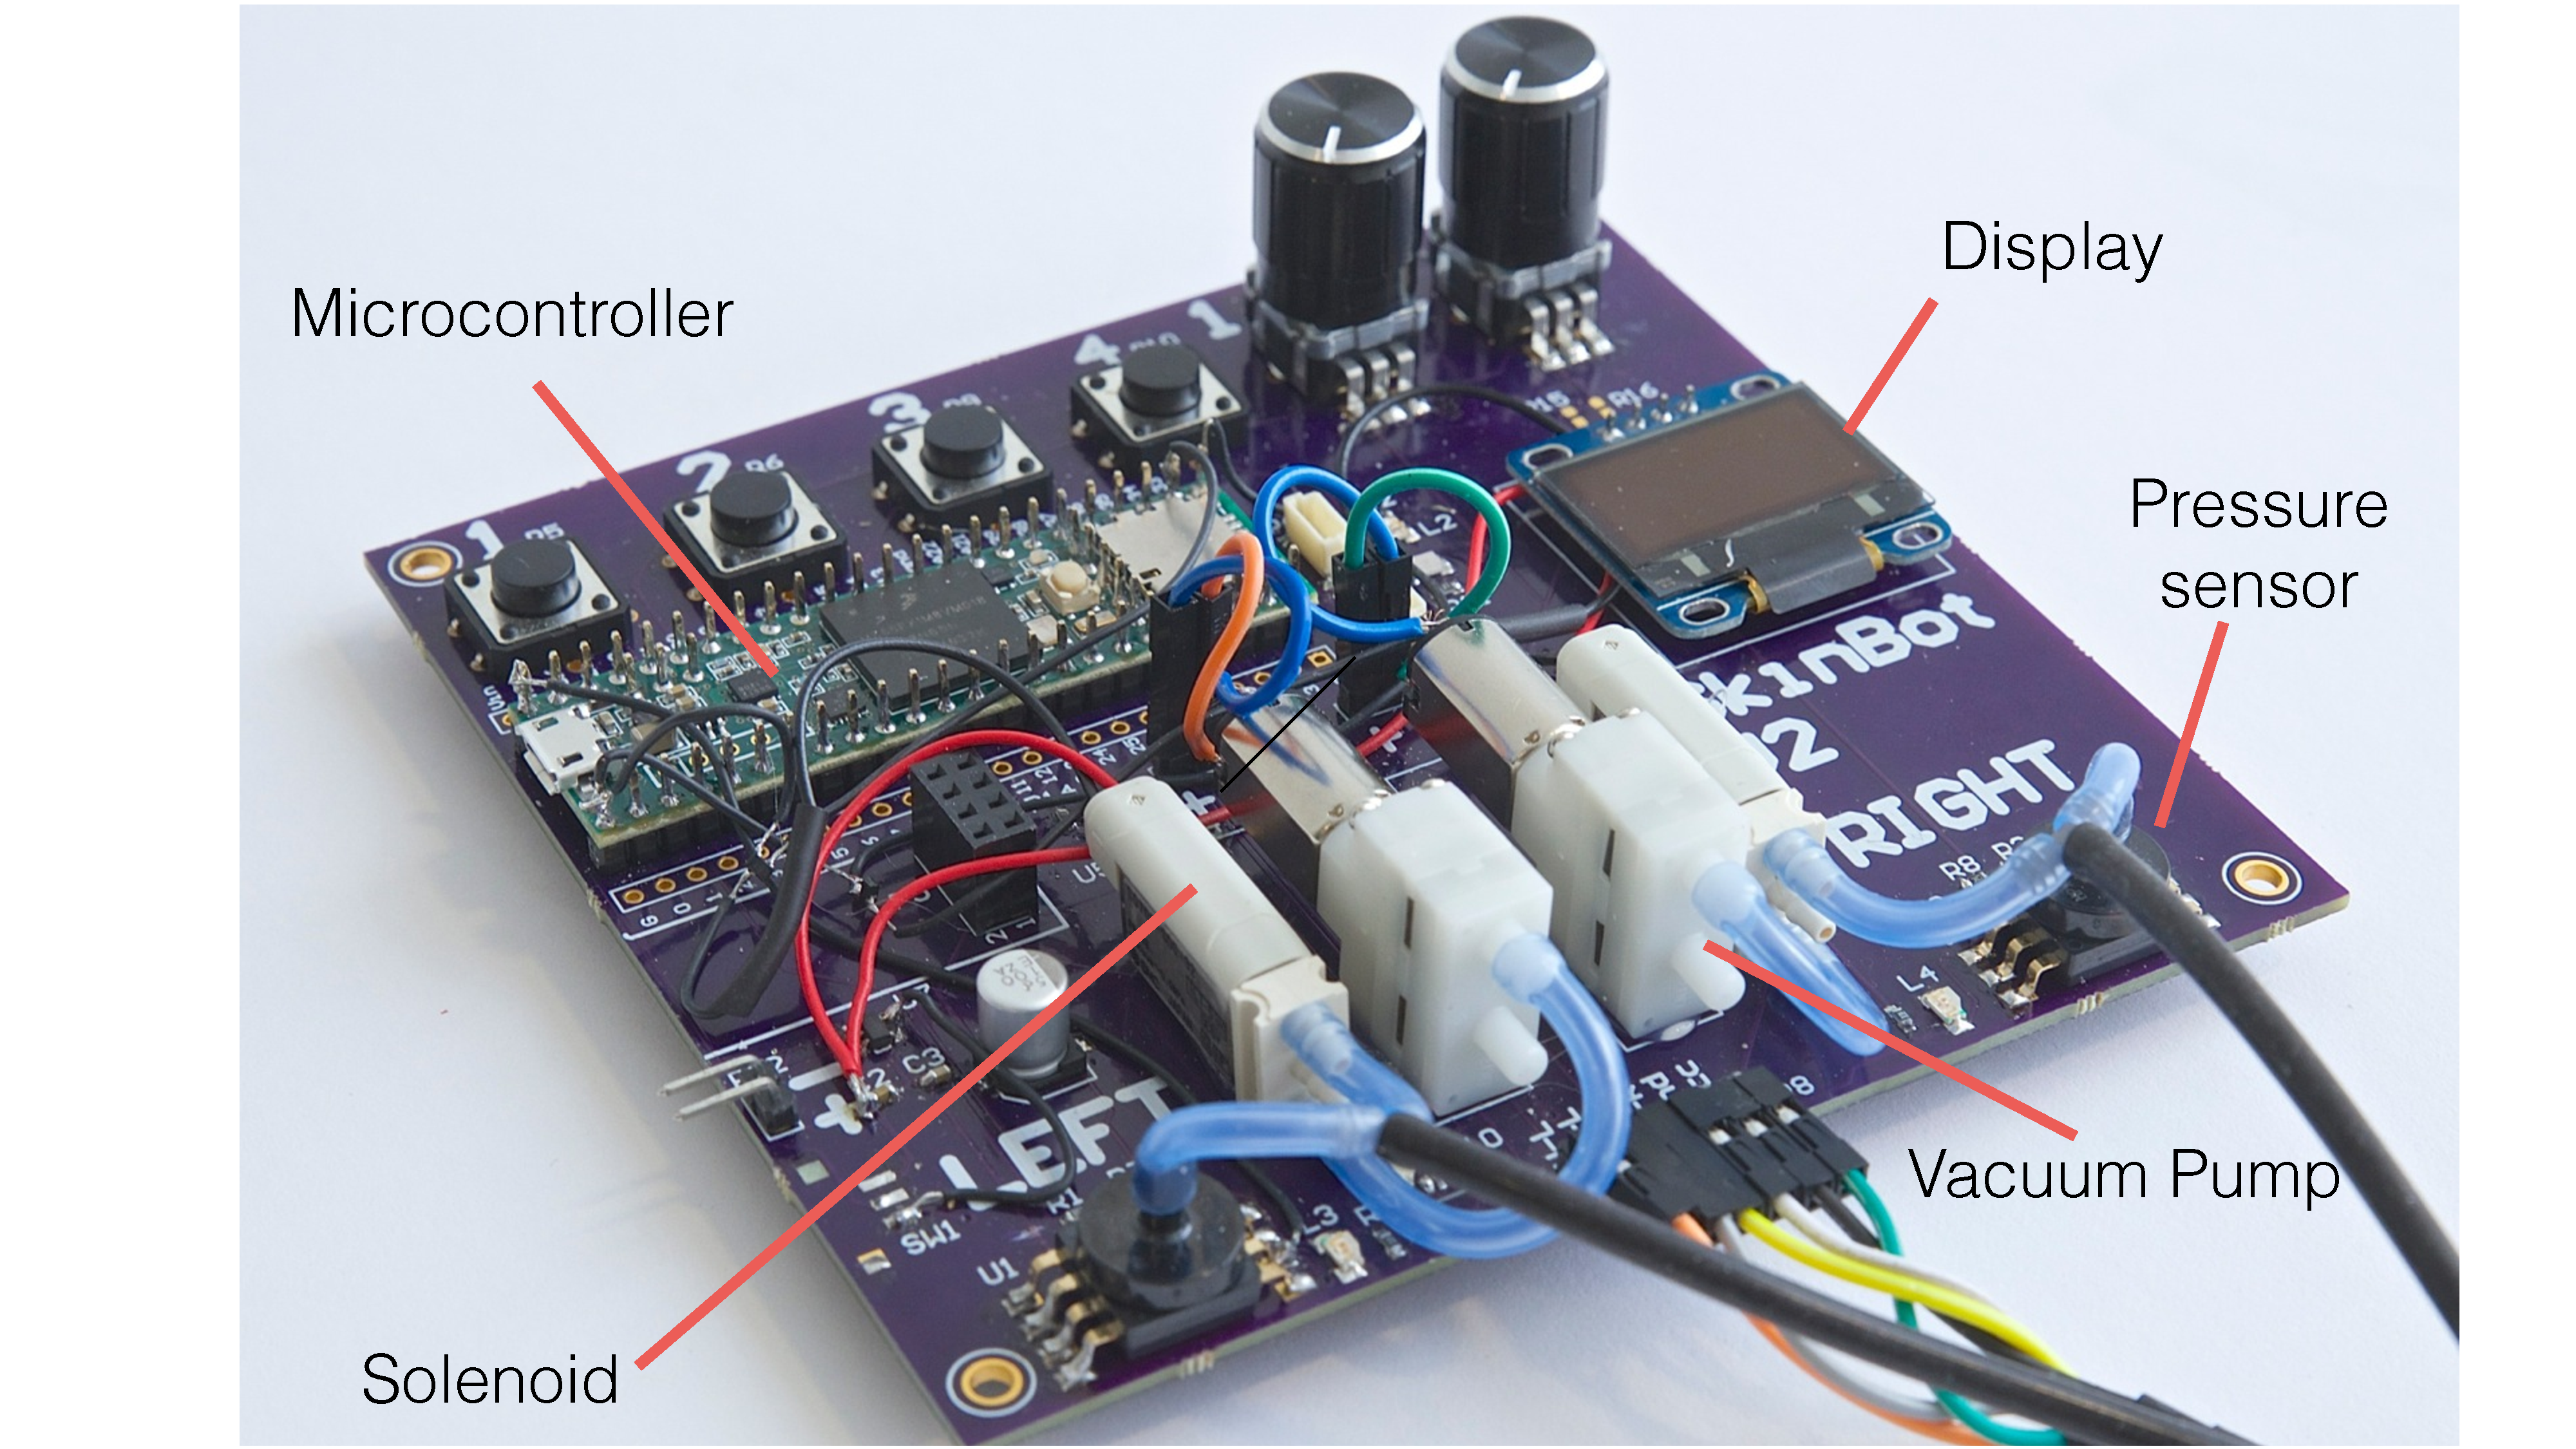
\includegraphics[width=8.0cm]{pictures/chapter3/master_node.pdf}
\caption{The master circuit board image. This board contains all the components required to run the tethered robot. The master board connected to the computer through the USB for communications and programming. The pumps, solenoids and servo motors run off separate power supply at 3.3V}
\label{fig:master_node}
\end{figure}



\begin{figure}[!t]
\centering
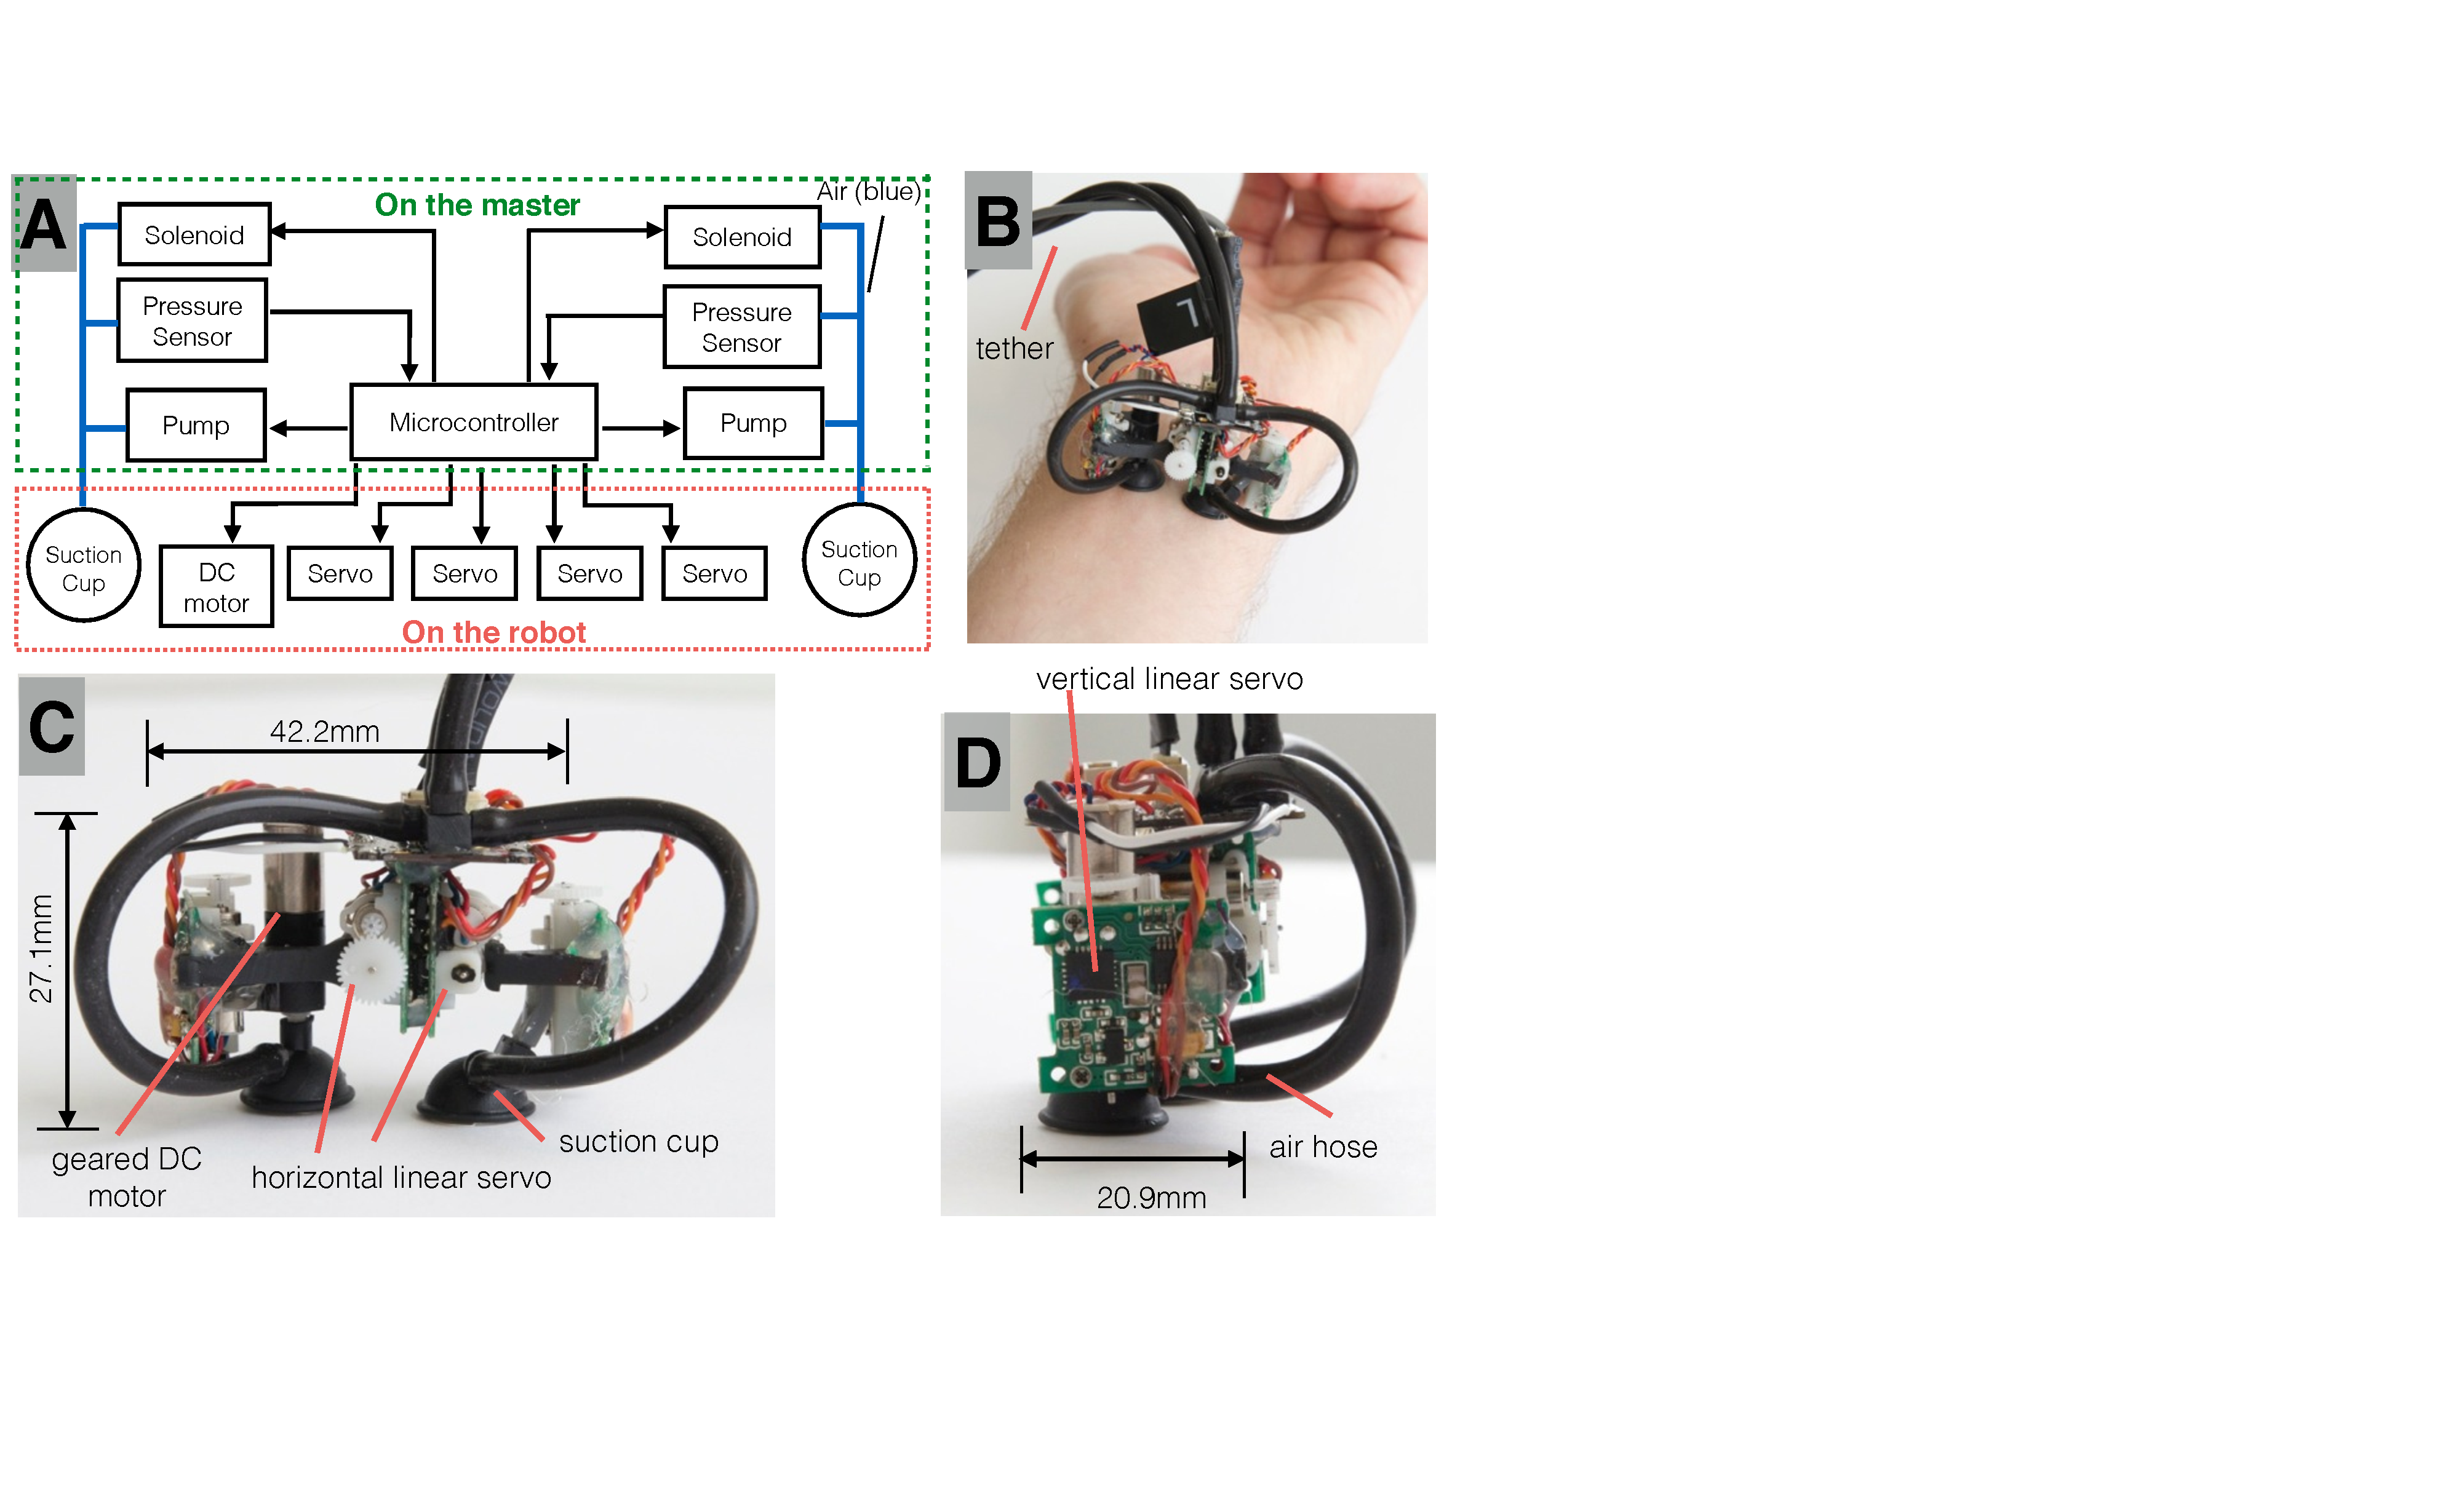
\includegraphics[width=12.0cm]{pictures/chapter3/robot_design.pdf}
\caption{SkinBot design. A)~The system diagram of the main components of SkinBot. B)~Robot attached to the arm. C)~The front of the robot. The robot combined four linear servo motors and DC gear motor to allow translation and rotation. D)~The side view of the robot.}
\label{fig:system_diagram}
\end{figure}


\section{Soft epidermal robots}
This section briefly describes the current and future direction of the soft epidermal robot. We found multiple problems with the current rigid robot design. The rigid robot has limited degrees of freedom. Also, the robot would break if it gets squished, which can happen if a person rolls over during sleep. To have multiple degrees of freedom as well as the resilient structure we created a prototype of a soft epidermal robot. The soft robotics has become a popular research topic and has a promising future, especially for robots that are near humans. I initially became involved in soft robotics as we looked at how to integrate airpouch-based actuators inside flexible circuit boards~\cite{dementyev2018mass}. 

\begin{figure}[!t]
\centering
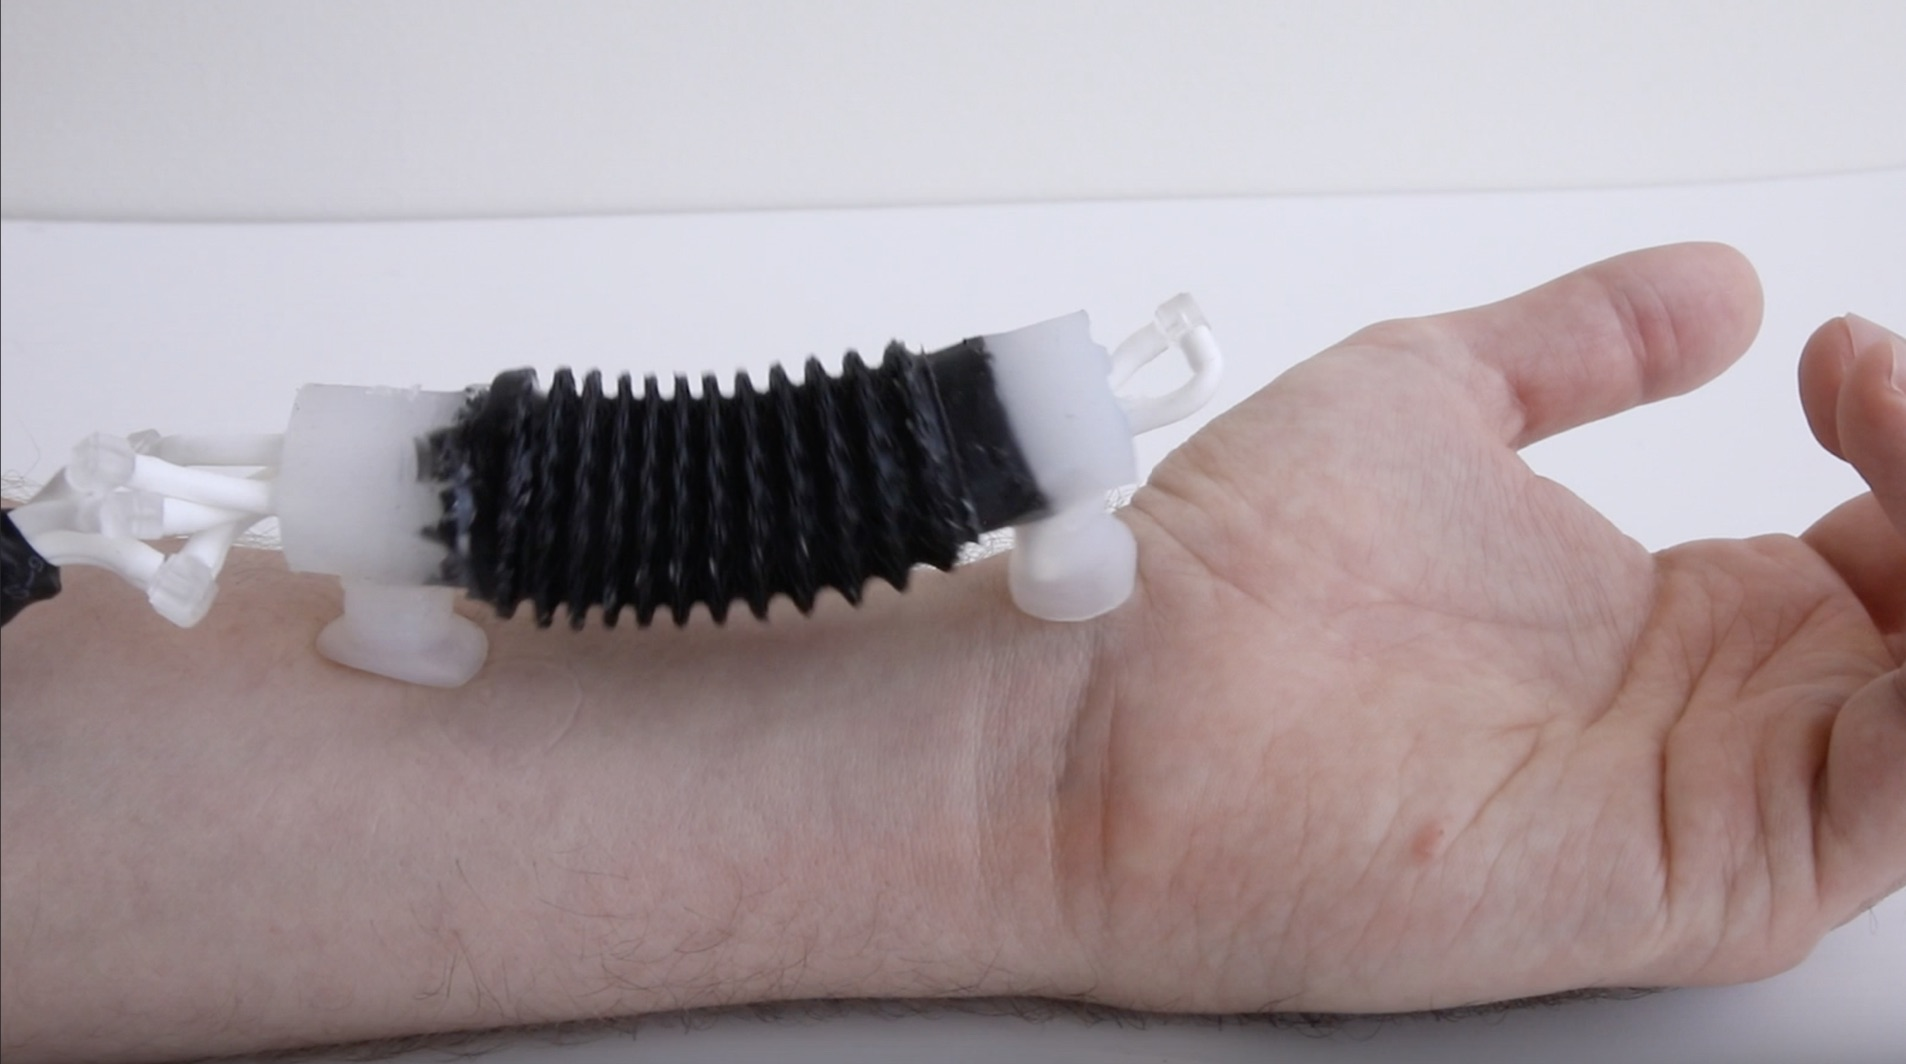
\includegraphics[width=12.0cm]{pictures/chapter3/soft_robot.jpg}
\caption{An image of the soft robot prototype}
\label{fig:system_diagram}
\end{figure}


\subsection{Design}
The robot design is based on the multi-module variable stiffness manipulator~\cite{de2017soft}. Using three air pouches this design can bend and elongate in any direction.  

\subsection{Manufacturing}
We primarily used a FDM 3D printer (Prusa) to make the molds for silicone. We attempted to use SLA printer but found that the resin can contaminate the silicone and inhibit curing. We used Ecoflex 00-30 as primary material, as it could expand when inflated. We also used Dragon Skin 30 for stiffer parts. 
Pictures of manufacturing and steps. 

\subsection{Discussion}
Some measurements about forces and speed. 

\section{Summary}
This work demonstrates the first epidermal robot with the ability to move over the surface of the skin and capture a large range of body parameters. We identified and met five critical design considerations for epidermal robots: lightweight and small, have access to the skin, have the ability to adhere and locomote, and provide multimodal sensing. We found that suction-based locomotion worked better than adhesive-based methods. The main challenge of skin climbing was the adhesion of the end effector (suction cup) to a new position. In our solution, we used a feedback approach, with pressure sensors and servo motors to attach to complex surfaces. Also, we probe a future direction of Epidermal robots by looking into soft robotics.

